\chapter{Results} \label{results}
This section will first describe the results from the experiments.

\section{Result Exhaustive Search}
    
    \subsection{Training}
        In figure \ref{training_overveiw_fig} an example plot in illustrated of how the training process was monitored. This example is small, but the most important features will now be described. The example comes from the final logging of the model trained on all frequencies.
        \clearpage
        \begin{figure}[H]
             %scale=0.4,

            \hspace*{-3.2cm}
            \includegraphics[scale=0.45]{figures/epoch_50_test_38kHz_18kHz_70kHz_120kHz_200kHz_333kHz.png}
            \caption[Training example monitoring]{Example training monitoring. The upper row shows the network's output for each class on a validation sample, with and without a threshold applied. In the lower row, the labels for each, with the historical loss and F1-score plots. Yellow is values close to 1 and purple is 0.}
          	\medskip 
            \label{training_overveiw_fig}
        \end{figure}
        
        
        Extracted from figure \ref{training_overveiw_fig} figure \ref{loss_f1_duo_plot_fig} illustrates both validation and the training follows the same values and convergence trend. The F1-score for validation and training data follows the same approximately same values, showing no issues regarding over-/under-fitting. Finally, the sanity check visualize good performance on correctly identifying \textit{sandeel} class as illustrated in figure \ref{sandeel_threshold_label}.%(add more examples to appendix?) 
        
        \clearpage
        \begin{figure}[H]
            \centering
            \subfloat[\centering Loss visualized along the y-axis and the x-axis represent epochs.]{{\includegraphics[width=5cm]{figures/Loss_val_train.png} }}%
            \qquad
            \subfloat[\centering F1-score visualized along the y-axis and the x-axis represent epochs.]{{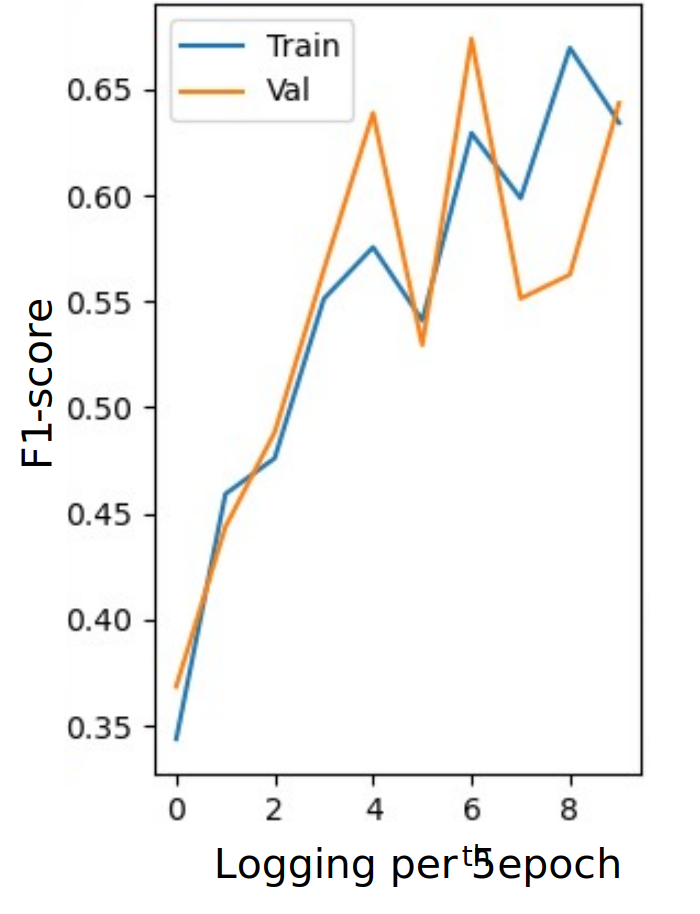
\includegraphics[width=5cm]{figures/F1_score_per_5.png} }}%
            \caption[Loss and F1 score during training]{The F1-score and loss for both training and validation. The validation loss was calculated less often, resulting in larger jumps in value. The training and validation F1-score on the final validation data was respectively 0.63 and 0.64.}%
            \label{loss_f1_duo_plot_fig}%
        \end{figure}
            
        \begin{figure}[H]
            \centering
            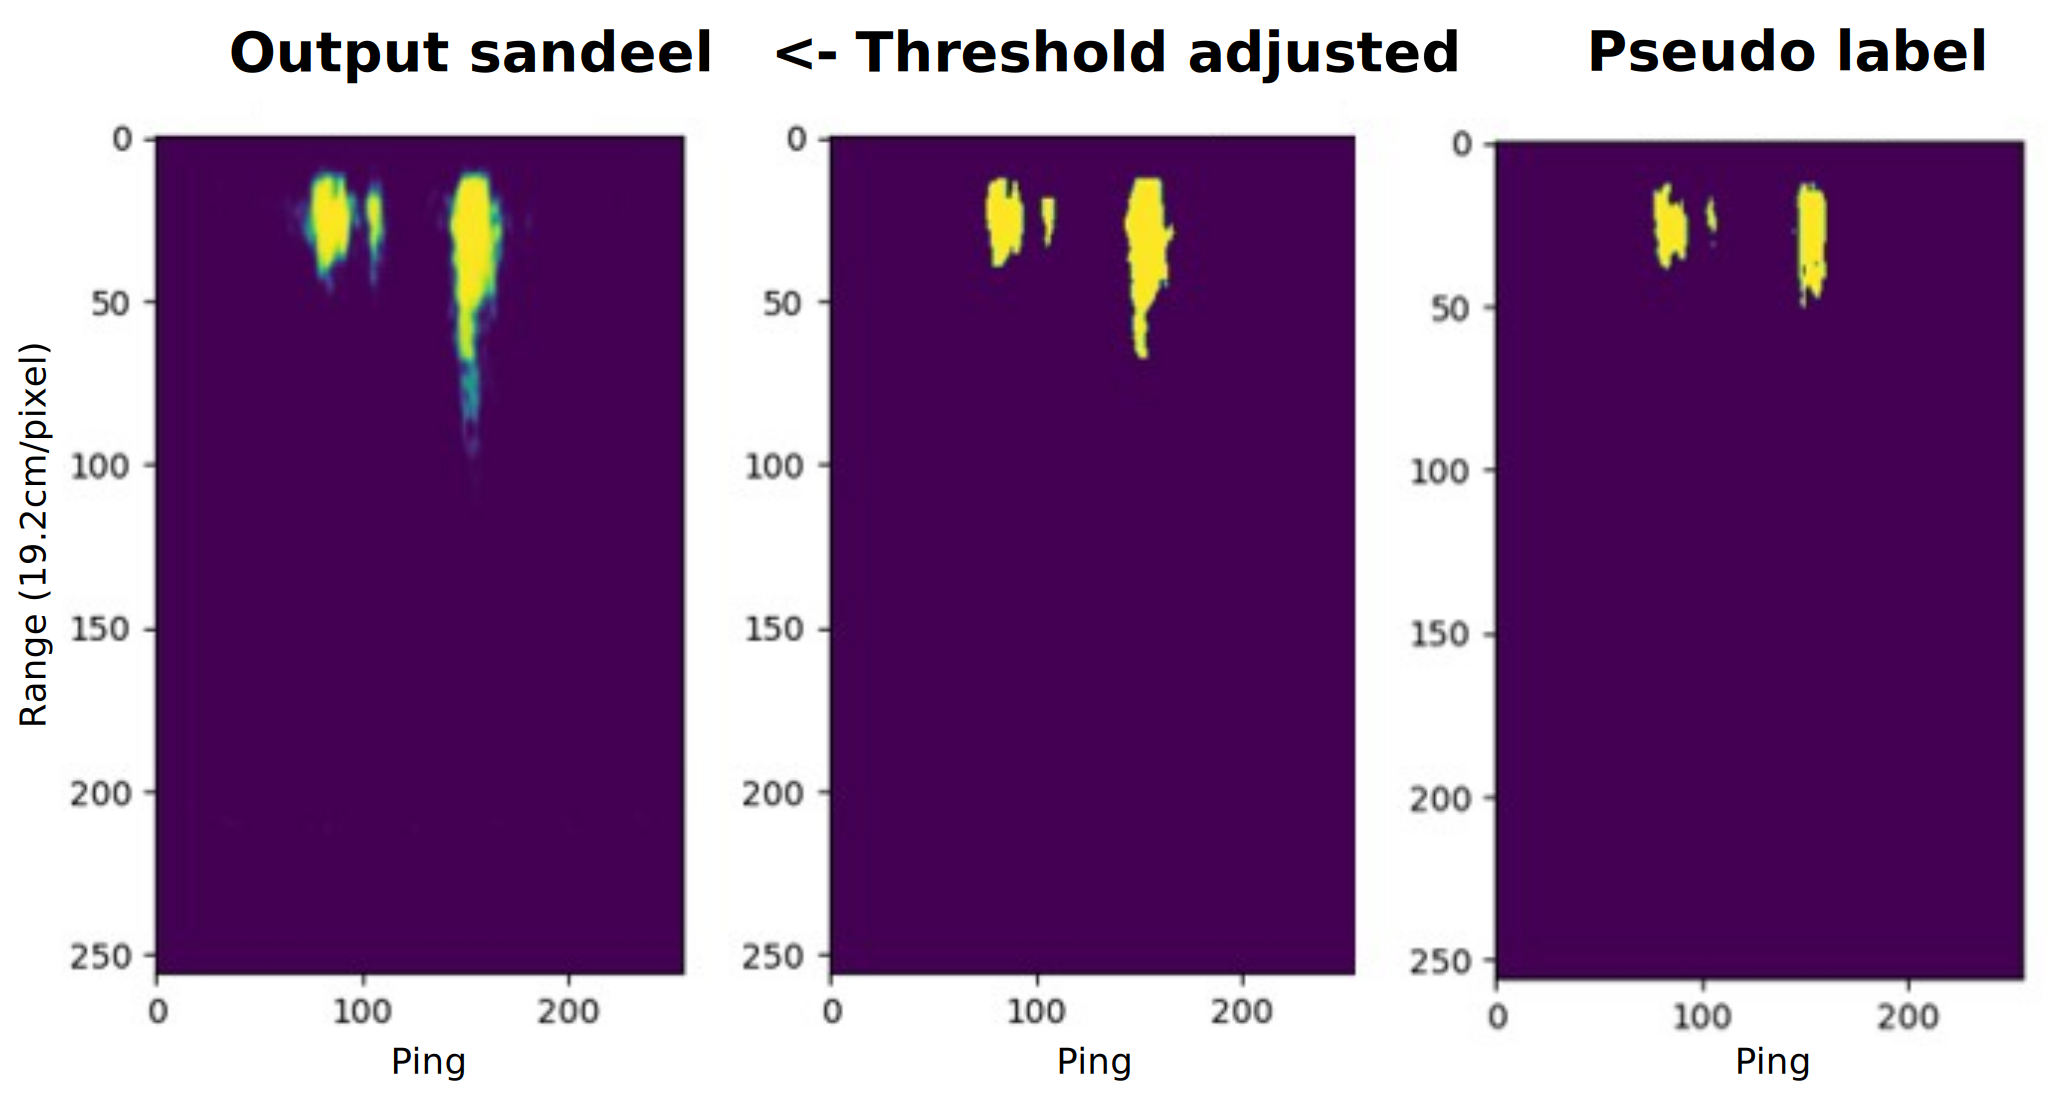
\includegraphics[scale=0.6]{figures/SANDEEL_WITH_LABEL.png}
            \caption[Examle output, threshold and label]{From left to right; Network output for the class \textit{sandeel}, same output threshold adjusted and finally the label for the current sample.}
          	\medskip 
            \label{sandeel_threshold_label}
        \end{figure}
    
    
    These results also show that a model can successfully be trained on pseudo labels. The logs from training showed that some combinations with low amounts of frequencies would need more training to converge. More examples on logged output can be found in the appendixes, as there are too many to efficiently illustrate here.  (LEGG IN DETTE). 
    
    \subsection{Performance Metrics - Greedy Search}
        In figure \ref{increasing_freq_f1_score_fig} the best frequency combinations based on F1-score is visualized. \textit{200kHz} dominates the results, and stays in all combinations. The most drastic increase in performance happens with the 3 frequencies \textit{18kHz}, \textit{38kHz} and \textit{200kHz} being used.
        \begin{figure}[H]
            \centering
            %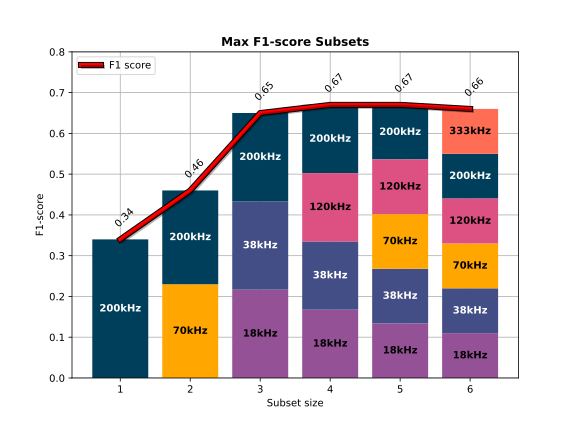
\includegraphics[scale=0.7]{figures/increasing_freq_f1.png}
            \includesvg[inkscapelatex=false,width=0.9\textwidth,keepaspectratio]{figures/increasing_freq_f1.svg}
            \caption[Best frequency combination - F1-score]{Colored blocks indicate the frequency or frequencies resulting in the highest F1-score in each tier of combinations.}
          	\medskip 
            \label{increasing_freq_f1_score_fig}
        \end{figure}

        In figure \ref{increasing_freq_precision_score_fig} the best frequencies combinations based on precision is visualized. The trend is similar to the one based on F1-score.
        % Precision
        \begin{figure}[H]
            \centering
            %\includegraphics[scale=0.7]{figures/increasing_freq_precision.png}
            \includesvg[inkscapelatex=false,width=0.9\textwidth,keepaspectratio]{figures/increasing_freq_precision.svg}
            \caption[Best frequency combination - Precision]{Colored blocks indicate the frequency or frequencies resulting in the highest precision in each tier of combinations.}
          	\medskip 
            \label{increasing_freq_precision_score_fig}
        \end{figure}
        
        In figure \ref{increasing_freq_recall_score_fig} the best frequencies combinations based on precision is visualized. The steep increase in performance happens already at two frequencies. Indicating that the best combination at this stage already finds most of the \textit{sandeel} class.
        %\clearpage
        \begin{figure}[H]
            \centering
            %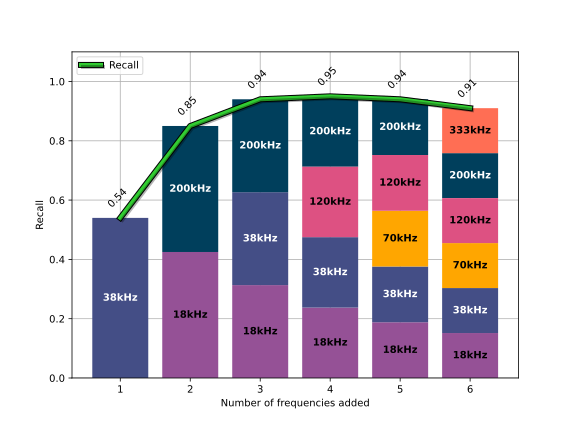
\includegraphics[scale=0.7]{figures/increasing_freq_recall.png}
            \includesvg[inkscapelatex=false,width=0.9\textwidth,keepaspectratio]{figures/increasing_freq_recall.svg}
            \caption[Best frequency combination - Recall]{Colored blocks indicate the frequency or frequencies resulting in the highest recall in each tier of combinations.}
          	\medskip 
            \label{increasing_freq_recall_score_fig}
        \end{figure}

    \subsection{All Combinations}
        Figure \ref{errorbar_fig} illustrate a complete plot of all error bars, with sections for each test. The plot has no complete overview over what frequencies belong to what result, but only a red circle encompassing the error bar related to the combination \textit{18},\textit{38} and \textit{200kHz}. This combination outclasses all other combinations in the same and previous tests, as well as competes with all the results later achieved. In all other sections, no combinations stands out as the unique regarding F1-score.
        
        \begin{figure}[H]
            \centering
            %\includegraphics[scale=0.7]{figures/error_bar.png}
            \includesvg[inkscapelatex=false,width=1\textwidth,keepaspectratio]{figures/error_bars.svg}
            \caption[Error bars per combination]{Each colored error bar is a frequency-combination. The error bar's top y-value value is the max value achieved, and the bottom is the lowest. A red circle encompasses the test containing only 18kHz, 38kHz and 200kHz. Blue vertical lines sections the error bars into groups where the number of frequencies in each combination are equal.}
          	\medskip 
            \label{errorbar_fig}
        \end{figure}
        
        
        
    \subsection{Performance Trend Per Frequency} 
        Figure \ref{performance_trend_fig} illustrates the performance trend of each frequency. From right to left, the plot shows to that \textit{18kHz}, \textit{38kHz} and \textit{200kHz} all are part of many combinations with high F1-scores. The rest quickly fall in performance, most likely due to not being paired with any of the three previously mentioned. Looking further to the left, \textit{18kHz} seems to have participated in many combinations on average, resulting in high F1-scores. Followed closely by \textit{200kHz}.
        \begin{figure}[H]
            \centering
            %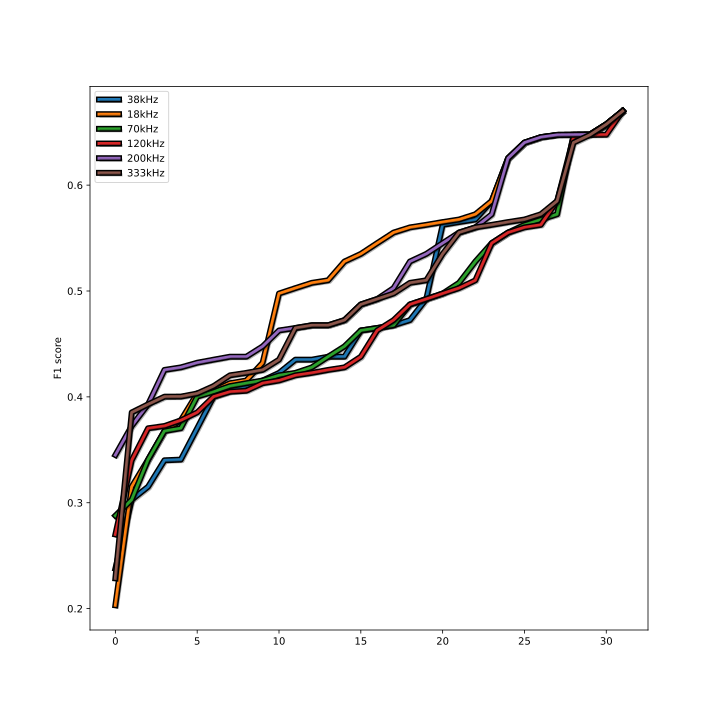
\includegraphics[scale=0.7]{figures/perfomance_trend.png}
            \includesvg[inkscapelatex=false,width=1\textwidth,keepaspectratio]{figures/perfomance_trend.svg}
            \caption[Performance trend per frequency]{For all combinations containing a certain frequency, the performance is plotted increasingly.}
          	\medskip 
            \label{performance_trend_fig}
        \end{figure}
        
        
    

    
    
